% !TeX encoding = UTF-8
% !TeX program = xelatex
% !TeX spellcheck = en_US

\documentclass[a4paper]{ltxdoc}
\usepackage{amsmath}
\usepackage[UTF8]{ctex}
\usepackage{unicode-math}
\usepackage{caption}
\usepackage{booktabs}
\usepackage{xcolor}
\usepackage{array}
\usepackage{listings}
\usepackage[perpage]{footmisc}
\usepackage{hypdoc}
\usepackage{geometry}
\usepackage{endnotes}
\usepackage{graphicx}
% \usepackage[multiple]{endnotes}
\usepackage{multicol}
\usepackage{listings}
\usepackage{hyperref}
\usepackage{blindtext}
\geometry{a4paper, scale=0.85}
\lstset{
    basicstyle          =   \sffamily,          % 基本代码风格
    keywordstyle        =   \bfseries,          % 关键字风格
    commentstyle        =   \rmfamily\itshape,  % 注释的风格,斜体
    stringstyle         =   \ttfamily,  % 字符串风格
    flexiblecolumns,                % 别问为什么,加上这个
    numbers             =   left,   % 行号的位置在左边
    showspaces          =   false,  % 是否显示空格,显示了有点乱,所以不现实了
    numberstyle         =   \zihao{-5}\ttfamily,    % 行号的样式,小五号,tt等宽字体
    showstringspaces    =   false,
    captionpos          =   t,      % 这段代码的名字所呈现的位置,t指的是top上面
    frame               =   lrtb,   % 显示边框
}
\lstdefinestyle{Python}{
    language        =   Python, % 语言选Python
    basicstyle      =   \zihao{-5}\ttfamily,
    numberstyle     =   \zihao{-5}\ttfamily,
    keywordstyle    =   \color{blue},
    keywordstyle    =   [2] \color{teal},
    stringstyle     =   \color{magenta},
    commentstyle    =   \color{red}\ttfamily,
    breaklines      =   true,   % 自动换行,建议不要写太长的行
    columns         =   fixed,  % 如果不加这一句,字间距就不固定,很丑,必须加
    basewidth       =   0.5em,
}


\title{针对ACG风格图像识别算法的一种改进和应用}
\author{少年班学院\ \ 马天开\ \ PB21000030}
\date{\today}

\begin{document}
\maketitle
\section{科学技术原理}
图像识别算法在近一个世纪以来都是深度学习的重要应用之一,在疫情期间也在部分场景中发挥了重要用途(比如 检查是否佩戴口罩、识别人脸及对应体温等)。

ACG风格是一种独特的绘画/美术风格,与现实照片相比,一般具有轮廓加粗、高对比度等特征。部分适用于现实照片的图像处理工具在ACG风格图片上可能出现准确率低、耗时更高的情况(尽管这类画风在理论上其实更容易被算法处理)。

\begin{figure}[h]
    \centering
    
\includegraphics[scale = 0.5]{img/ACG.jpg}
    \caption{ACG风格图像}
\end{figure}

我们从被广泛使用的\textit{Yolov5}算法开始,本着重造轮子的精神,对其训练和检测算法进行重构,并给出改进后算法的一个可行应用,以及应用背后的意义。

\subsection{\textit{Yolov5}模型简述}

\textit{Yolov5}模型相较于上一代很相似,还是分为输入端、Backbone、Neck、Prediction四个部分。
\begin{figure}[h]
    \centering
    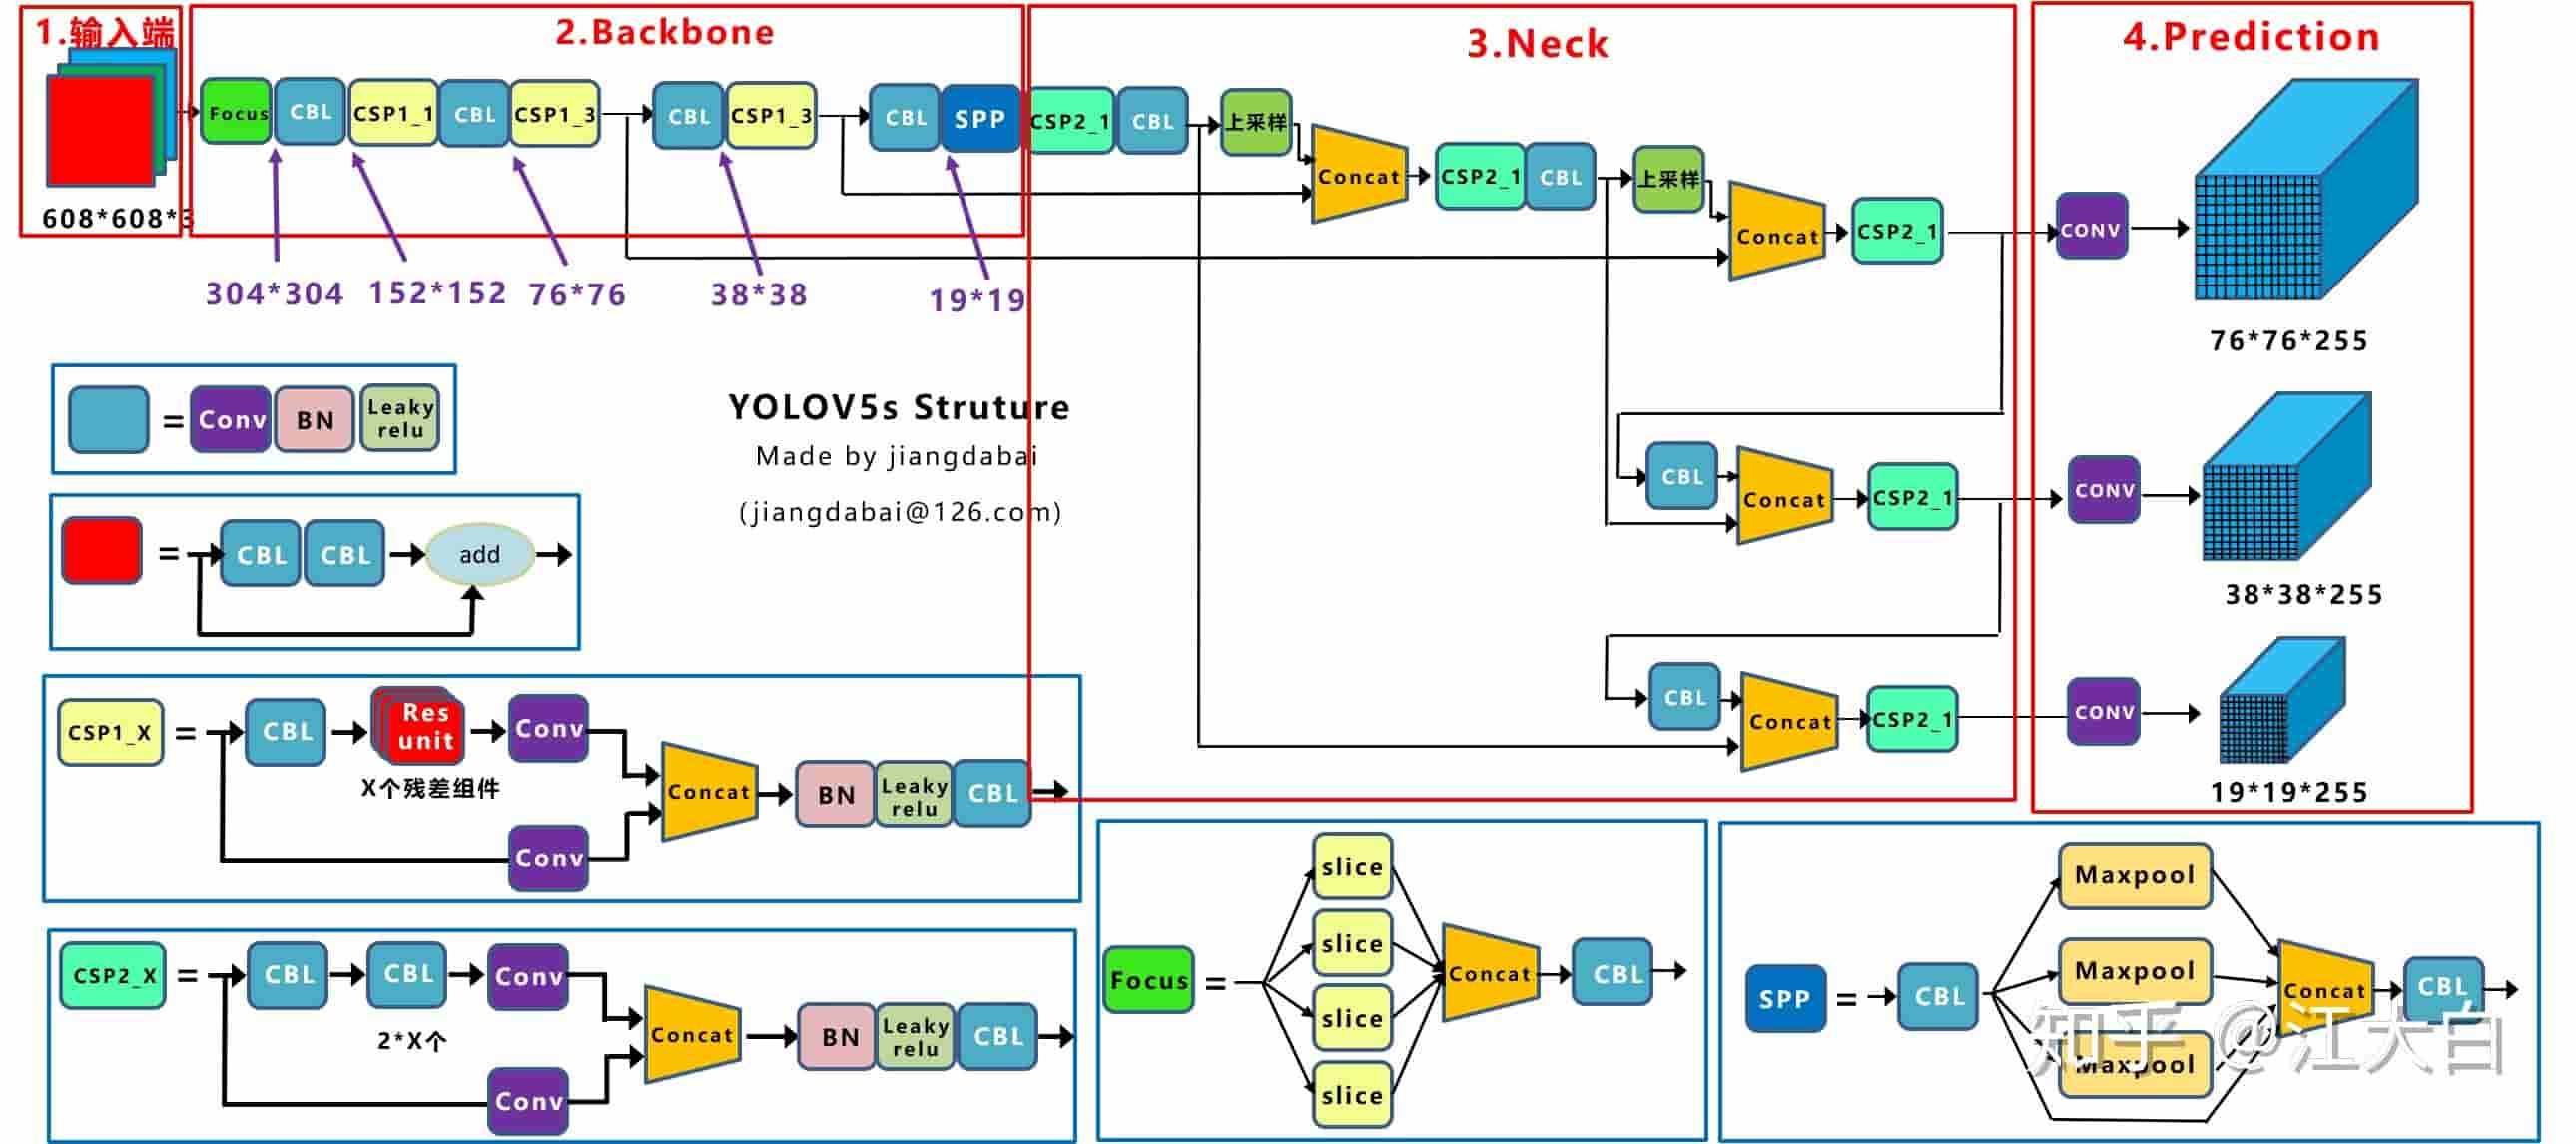
\includegraphics[scale = 0.1]{img/yolov5.jpg}
    \caption{Yolov5模型}
\end{figure}

其中,在本项目中,相较于\textit{Yolov4},提升最大的地方在于自适应锚框计算和图片缩放上。

另外,在\textit{dataset.py}中,\textit{Yolov5}给出了新的缩放算法,减少了缩放图片时两侧的黑边,将推理速度提升了37\%。

\subsection{改进思路}

针对ACG这种不算复杂的图像,\textit{Yolov5s}能在保证精度的前提下最大化提升推理推理速度,在此基础上,我们再略微提升一点精度,便可达到更大的平衡。

在模型训练上,加入了\textit{Mosaic}数据增强方式,提升了鲁棒性。同时删除了模糊增强的部分,改为GrayScale的方式,提升颜色分块在训练结果中的作用。

\begin{lstlisting}
    if self.augment:
        img, labels = self.albumentations(img, labels)
\end{lstlisting}

同时,上文提到的\textit{letterbox}函数也可以进一步优化(前后对比发现,过度缩放会带来训练精度的显著降低),改为以下逻辑:

\begin{lstlisting}
    shape = im.shape[:2]
    if isinstance(new_shape, int):
        new_shape = (new_shape, new_shape)

    r = min(new_shape[0] / shape[0], new_shape[1] / shape[1])
    if not scaleup:
        r = min(r, 1.0)

    ratio = r, r
    new_unpad = int(round(shape[1] * r)), int(round(shape[0] * r))
    dw, dh = new_shape[1] - new_unpad[0], new_shape[0] - new_unpad[1]
    if auto:
        dw, dh = np.mod(dw, stride), np.mod(dh, stride)
\end{lstlisting}

\subsection{应用思路}

经过改进后,在样本量为300的(采集自Pixiv的图片),针对识别\textbf{眼镜}这一主体,精度可以维持在$97.3\%$(训练集大小:$20$,$epoch = 40$)

为更直观地展示改进后算法的能力,我选择了一个对延迟、精度都很敏感的场景:音乐游戏。(简单来说就是需要在指定时间,根据屏幕提示,按下特定按键的场景)

为此,适配了\textit{Windows}平台下模拟按键的脚本,并完成了从识别到点击的拟合逻辑(多帧线性插值)。

项目演示地址:\url {https://www.bilibili.com/video/BV1NU4y127rH/}

\begin{figure}[h]
    \centering
    
\includegraphics[scale = 1]{img/qrcode.png}
    \caption{演示地址}
\end{figure}

\section{设计方案}

复现项目的主要过程为:

\begin{itemize}
    \item 提取数据,并将其转换为受\textit{Yolov5}支持的格式,类似的工作已经有机构做过非常方便的工具。\\ 参考\url {http://roboflow.com/}
    \item 训练数据,并使用\textit{Yolov5}模型进行推理,对应的文件为\textit{train.py},其中大部分代码为我重构的部分,小部分直接引用了\textit{Yolov5}源码。
    \item 打开游戏,同时打开脚本,此时脚本将会自动识别屏幕上出现的物体,自动帮助按下\textit{f}和\textit{j}键,以完成游戏。
\end{itemize}

按照实际使用的顺序,程序的大致结构为:

\begin{itemize}
    \item \textit{\backslash utils},此目录包含训练时绝大部分所需要使用的script,其中较为突出的时\textit{activations.py}作为激活函数,\textit{loss.py}评估损失函数
    \item \textit{\backslash models},此目录为\textit{Yolov5}拷贝的内容,用于导出训练结果。
    \item \textit{train.py}用于训练新模型,\textit{key\_win.py}用于模拟Windows下键盘输入。
\end{itemize}

\section{创新性描述}

目录下除\textit{\backslash models},以及\textit{utils/loggers}为\textit{Yolov5}拷贝的内容外,其余部分都是我自己独立完成或重构的代码。
在重构代码时,以不抄袭为原则,但部分实现较为单一或是没有第二种解决方案(或没有更优解时)可能存在重复。

项目的优点:

\begin{itemize}
    \item 针对ACG风格图像,对识别算法进行了一次改进
    \item 在应用上,能够直观地反映新算法带来的精度和效率的能力
    \item 更加直观地反映深度学习模型的能力
\end{itemize}

\section{运行方法和参数设置}

前提条件:PyTorch安装,并且推荐的配置为:Ryzen 9 5900HX + NVIDIA RTX 3070起步,单独使用CPU的训练时间极长,$epoch$较小时训练效果不佳。

要复现本实验的结果,首先要整理一套完整的数据。为方便起见,可以参考\textit{fetch\_data.py}中的代码,这里面包含了我本次使用的数据集。

接下来是训练,可以用以下命令调用\textit{train.py}:

\begin{lstlisting}
    python train.py --img 640 --batch 4 --epochs 100 --data /path/to/data.yaml --weights yolov5s.pt
\end{lstlisting}

在训练推理结束时,可以用以下命令简单评估训练结果:

\begin{lstlisting}
    python .\detect.py --weights /path/to/best.pt --source /path/to/img
\end{lstlisting}

接下来,打开脚本和游戏(先后顺序无关,脚本会自动采集第一块屏幕的数据),在脚本识别到对应物体时,便会自动按下按键。

\section{学习心得和收获}

在本次课程之前,我对Python一直处在一个自己摸索、时常碰壁的学习路上。在最开始使用的时候更为严重,平均下来写代码和排查错误的时间大概要对半分。也不能很好地利用报错信息来排查错误,导致我最开始使用Python的体验相当不好,甚至我一度怀疑这样一门语言对效率的提升究竟有多大。

在本次课程之后,尤其是从课程一开始我就在搞的这个项目,逐渐锻炼了我排查错误、调试以及熟练查文档的能力。现在能达到几乎写C++效率的3~5倍,可以说真正地把Python当作一个有趣的工具来使用。也希望它能在日后的学习/工作中更大地发挥作用。

具体一点讲的话,在本次项目中收获最大的应该要数Anaconda和Pycharm的使用了。有趣的工具总是能带来更有趣的体验,在熟练使用之后,会比单纯使用VSCode的体验和速度更上一层楼。

同时,也是最大的帮助——更熟练了\textit{pyTorch}的使用,在日常使用\textit{tensorflow}的基础上,另一种工具的学习总是显得相得益彰。

\section{参考资料}

在目标检测上,参考了\url {https://zhuanlan.zhihu.com/p/454472695} 里面提到的\textit{Yolo}的检测方法。

YoloV5 模型的学习和理解参考了\url {https://zhuanlan.zhihu.com/p/143747206}及其下面的一些的文章,我对于模型的了解基本建立在这几篇文章和源码的基础上,在此表示感谢。

同时,参考了以下文献:

YOLOv3: An Incremental Improvement, Joseph Redmon \& Ali Farhadi, arXiv:1804.02767v1 [cs.CV] 8 Apr 2018

YOLOv4: Optimal Speed and Accuracy of Object Detection Alexey Bochkovskiy \& Chien-Yao Wang \& Hong-Yuan Mark Liao

在此一并表示感谢。
\end{document}